  % Gebäude: E1.3     Gebäude: E1.3  
  \documentclass[a4paper,11pt, openany]{book} %Remove draft option to hide ToDos

\include{header}
\tolerance=200

\settitle{Perceptions of privacy and control over Personal Data among Indian Internet Users}
\setauthor{Pavan Raviteja Upadhyayula}
\advisor{Dr. ir. Mannat Kaur \\ Dr. Ha Dao}
\reviewerOne{Prof. Dr. Anja Feldmann}
\reviewerTwo{Dr. Katharina Krombholz}
\university{Saarland University}
\faculty{Faculty of Mathematics and Computer Science}
\thesistype{Master's}
\subdate{01}{January}{2017}
\city{Saarbr\"ucken}
\setBaseUrl{{https://www. ... .de/coq/}}

\DeclareTextFontCommand{\emph}{\bfseries}


\pagenumbering{roman}

\setlength{\headheight}{15pt}

\pagestyle{fancy}
\renewcommand{\chaptermark}[1]{ \markboth{#1}{} }
%\renewcommand{\sectionmark}[1]{ \markright{#1}{} }

\fancyhf{}
\fancyhead[LE,RO]{\thepage}
\fancyhead[RE]{\textit{ \nouppercase{\leftmark}} }
\fancyhead[LO]{\textit{ \nouppercase{\rightmark}} }

\fancypagestyle{plain}{
	\fancyhf{}
	\renewcommand{\headrulewidth}{0pt}
	\renewcommand{\footrulewidth}{0pt}
}

%\makeglossaries

\begin{document}

\renewcommand\cite{\citep}

\thispagestyle{empty}

\maketitlepage

\statementpage

%\chapter*{Abstract}
%\addcontentsline{toc}{chapter}{\numberline{}Abstract}
%\input{abstract}

\newpage

%\chapter*{Acknowledgements}
%\input{acknowledgements}

\addtocontents{toc}{\vspace{5mm}}

\tableofcontents

%\listoftodos

\clearpage
\pagenumbering{arabic}

\chapter{Introduction}

Data breaches have grown exponentially, with over 1800 reported breaches in the first half of 2026, putting it on course to set a new annual record. AI has accounted for an increase of over 56\% of breaches from the previous year and with over 6 billion Internet users as of April,2026, placing the need for personal data governance at an all-time high at the moment. While newer regulations are constantly being adapted to ensure compliance, that hasn't hindered malicious actors from playing their hand and thereby affecting millions worldwide. This need for personal data privacy is further emphasized when large-scale infrastructural breaches such as the 2026 Canvas data breach occur, compromising 275 million users and their Personally Identifiable Information (PII) worldwide. While laws such as the General Data Protection Act (GDPR) in the E.U, the California Consumer Privacy Act (CCPA) in the USA and the Personal Information Protection Law (PIPL) in China have reinforced user data protection, enabling stricter regulations and tighter controls worldwide, their efficiency in dealing with the blurry lines has often come under scrutiny, especially with respect to their usage, adoption and understanding by lay-people. 

With a population of over 1.47 billion people, online penetration of 70\% as of October, 2025 and a new Digital Personal Data Protection Act (DPDPA) in partial enforcement from November, 2025, India is heading towards being a landmark example of digital privacy enforcement in de-centralized environments and also a certain opportunity for large-scale breaches with an existing evidenced past. This new act which was first passed in 2023, aims to reinforce India's digital landscape, focusing on the user's autonomy over their digital personal data, while providing lawful practices for organizations to process such data. Prior works on the Act discuss about the user's understanding of its laws and the need for such regulations. However, past research in aforementioned established contexts has shown that when such regulations are implemented without the consideration of the general population's needs and understanding, it could lead to frustration over certain practices, loopholes for organizations to bypass and overall skepticism on the implementation. 

Considering that the DPDPA is heading towards a complete enforcement and compliance from all the organizations from November, 2026, it is therefore important that the users' perspectives on their personal data privacy, sensitivities of various personal data items and their processing be understood to get a holistic perspective of the actual needs that need to be fulfilled and protected by the Act. This is especially important given that research has found users to emphasize the importance of their financial data in the past but haven't paid much heed to any other forms of personal data, which could potentially lead to their profiling and misuse by exploitative companies or practices. Additionally, given the recency of the Act, and its provisions to provide the users with the option to request collected data and consent revocal for its processing, it is especially important to understand their perspectives on such personal data processing and their perceived control throughout the process. While many legal experts have discussed and dissected the Act's vague definitions and their implications, an understanding on the possible gap between the user's perceptions of such definitions and process to the actual provisions of the Act would therefore establish a baseline comparative differentiation to rely upon. 

To address these gaps, an exploratory survey of 239 primarily educated participants with potential familiarity of online spaces was conducted. The analysis focused on the end user's perspectives of their general privacy perceptions of their personal data, their perceived sensitivity of the various personal data items and their perceived control over such data's processing. The study focuses on providing an initial understanding of the user's perceptions over this entire process, thereby understanding their (mis)alignment with the provisions of the Act. To do so, the following research questions were addressed:

\begin{enumerate}
    \item What are Indian Internet users’ perceptions about the privacy-sensitive nature of different types of personal data?
    \item What are Indian Internet users' beliefs regarding their control over different types of personal data and its processing?
\end{enumerate}


\chapter{Relevant Literature}

The term \textit{Privacy} by definition can be categorized in a broad manner, without explicitly ever encountering the actual depths of what it means to an individual. This complexity increases when the ideologies of culture is borrowed and intertwined in this context, to help understand the nuances of the environments it exists within. Such nuances have a lasting impact in the way people perceive the privacy of one's self, depending on the context that is being considered. Personal data privacy therefore, should ideally incite the strongest reactions of protection and safeguarding, since it involves dealing with information which is closest and dearest to the user with respect to their everyday lives. Past works \cite{zou_ive_nodate, mayer_now_nodate, karunakaran_data_nodate} however, show us that while the users display mixed awareness about the breach of their personal data privacy, more often than not they believed that the breach would not impact them in any reasonable manner. This elicits a notion of 'Privacy Paradox' \cite{acquisti_economics_2016}: people claiming that they are concerned about their privacy but often not taking measures to safeguard it. 

Regulations such as GDPR and CCPA were introduced to help the users by providing the necessary safeguards to take control over the provision, processing, and usage of their personal data by various organizations. While there was some initial skepticism towards the effectiveness of the individual claims and rights by the public \cite{strycharz_data_2020}, they were hopeful in terms of the implementation of such safeguards and maintained that it would eventually lead to more privacy-focused infrastructural developments \cite{mangini_empirical_2020}. Although the intention was to help the masses have an understanding over their control and rights, it has not translated into actual privacy practices. This left the users having a lack an understanding of the privacy disclosures due to the ambiguity on why their data is being collected \cite{chen_fighting_2021}, alternative ways for organizations to be notoriously hidden with their data practices \cite{oconnor_clear_2021}, disclosure of irrelevant information and overwhelming the users when they explicitly want practices to be transparent and fair. \cite{kyi_it_2024}. 

Schomakers et al. \cite{schomakers_internet_2019} compared the privacy perceptions of German users with those from the Brazilian and the US contexts, to understand if there any differences in their perspectives on the sensitivities of the different data items. They observed that although the ranking remained similar across the nations, there were differences in terms of the associated risks involved in disclosure of such information and how these could possibly be explained by factors such as habits, education level and privacy disposition. Similarly, Herbert et al. \cite{herbert_world_2023} conducted a large-scale longitudinal survey to understand if demographic factors played a role in the way that people held misconceptions about various security and privacy practices. They noticed that the country of residence played a key role in withholding such beliefs, while also suggesting the possibility of Internet literacy or technological readiness influencing the participants. Herbert et al. \cite{herbert_digital_nodate} also conducted another study using this same dataset, to understand the differences in the digital security \& privacy perceptions and practices of participants from WEIRD vs NON-WEIRD countries, focusing on their sensitivity of various data items, risks by possible attackers, previous experiences etc. They found that participants from non-WEIRD countries scored higher on all their measurement variables showcasing higher awareness, perception and exposure in terms of their security practices. One of their key findings was that the non-WEIRD participants relied heavily on their friends and family for digital security advice, which showcases a communal perspective towards these practices.

In an identical notion but with a qualitative perspective, Umbach et al \cite{umbach_your_2023} compared user perceptions on their security \& privacy practices of participants from Brazil, Philippines, India, Egypt and Nigeria. They found that one of the primary concerns of the participants revolved around their financial data and being wary of scammers in this regard, while also talking about their device-sharing methods obstructing with their individual right to privacy. This behavior was also noted across other contexts with Ahmed et al. \cite{ahmed_everyone_2019, ahmed_digital_2017} finding that while economic need is driving factor in device-sharing, it also stems from deep-rooted social and cultural practices in the Bangladeshi societies. They also found that existing power dynamics and patriarchal practices were also amplified due to this practice, thereby revealing its impact on the women's privacy autonomy in the society. Such dynamics and power structures in the context of personal data privacy was even more prevalent in the Arab Gulf, where Abhokhodair et al. \cite{abokhodair_privacy_2016, abokhodair_photo_2017} observed that decision making on Social media and Photo-sharing platforms involved not just the user's concerns of their safety and privacy but also an adherence to their religious and societal beliefs. In an almost similar environment, Naveed et al \cite{naveed_ask_2022} conducted interviews with Pakistani users from low-literacy, low-income backgrounds regarding their privacy choices and its implications on their personal data. They echoed similar sentiments of religious and societal beliefs of patriarchy playing a key role in especially impacting the women's management of privacy choices and control on their 'personal data'.

Kumaraguru et. al \cite{kumaraguru_privacy_2012} conducted an empirical study on the user perceptions of their privacy choices with a sample of 10,427 participants across India, and found that the participants were split in their opinions on what constituted as personal data and thereby more sensitive and private in nature. They also observed that the participants were considering financial data to be one of the most important forms of personal information, due to their awareness of the various financial scams. However, this work was conducted in 2012, making the results non-replicable given the growth of Internet penetration, awareness as well as the changes in the judicial aspects with respect to personal data privacy of the country since that time period. Recent works focused more on specific aspects of user privacy perceptions such as: Privacy practices of older house members and their families \cite{murthy_individually_2021}, Security and Privacy of UPI users \cite{mungara_security_nodate}, Geosocial Networking apps and the navigational challenges involved in them while safeguarding one's privacy \cite{pinch_someone_2022}, low-income users and their challenges to safeguard their privacy while navigating the identity infrastructure \cite{srinivasan_poverty_nodate}, low-income new Internet users and how they navigate through the realm of privacy \cite{popuri_i_nodate} and User's attitudes on AI sources \cite{kapania_because_2022}. 

Almost of these works dealt exclusively on specific aspects of user privacy perceptions or were conducted in specific contexts. Given the recency of the DPDPA's partial enforcement, it is therefore necessary to understand user privacy in the context of their personal data and how it is perceived. Priyadarsini et al. \cite{patil_web_2025} focusing primarily on the user's web privacy perceptions did touch this topic slightly, finding out that in their sample size, the participants were skeptical about sharing personal data like financial information and were more aware of sharing it on social-media applications than on e-commerce platforms. Additionally, Athar et al. \cite{10.1145/3779208.3785287} tried to understand the participant's interactions with cookie banners and how they perceived some of the laws of the DPDPA. They observed the possibility of 'privacy paradox' being present within their responses and an overall sentiment of distrust in the government's application of the Act. However, it is evident that while there has been extensive research done in the Indian ecosystem with regards to the user privacy perceptions, there has not been any work done focusing solely on user privacy of their personal data and its processing which is the primary focus of this Act. To the best of my knowledge, this is the first work which tries to understand the general privacy perceptions of the user with respect to their personal data along with their sensitivities of the various personal data items, helping us understand if there is a mismatch in the user comprehension aspect to what the Act is expected to cater. Minimizing this mismatch, could help in the progression of this Act to a wider community, thereby serving its purpose to the fullest.




\include{chapterThree}

\appendix

\addtocontents{toc}{\vspace{5mm}}

\chapter{Appendix}

\section{Adapted IUIPC Scale (Section - 1)}
\label{Adapted_Survey}
\textbf{Control:}
\begin{enumerate}
    \item I believe my personal data online should be under my control, and I should decide how it is collected, used, and shared
    \item Having control over my personal data is the key to my online privacy
    \item I believe that my online privacy is violated when my personal data is used without my consent or knowledge
\end{enumerate}

\textbf{Awareness:}
\begin{enumerate}
    \item Online companies should clearly explain how they collect, process, and use personal data
    \item Privacy policies should be clear and easy to understand
    \item It is not important for me to know how and why my personal data is being used
\end{enumerate}

\textbf{Collection:}
\begin{enumerate}
    \item It usually bothers me when online companies ask me for personal data
    \item When online companies ask me for personal data, I sometimes think twice before providing it
    \item It does bother me to give personal data to so many companies
    \item I am concerned that online companies are collecting too much personal data about me
\end{enumerate}



\section{Poster}
\label{fig:poster}
\begin{figure}
    \centering
    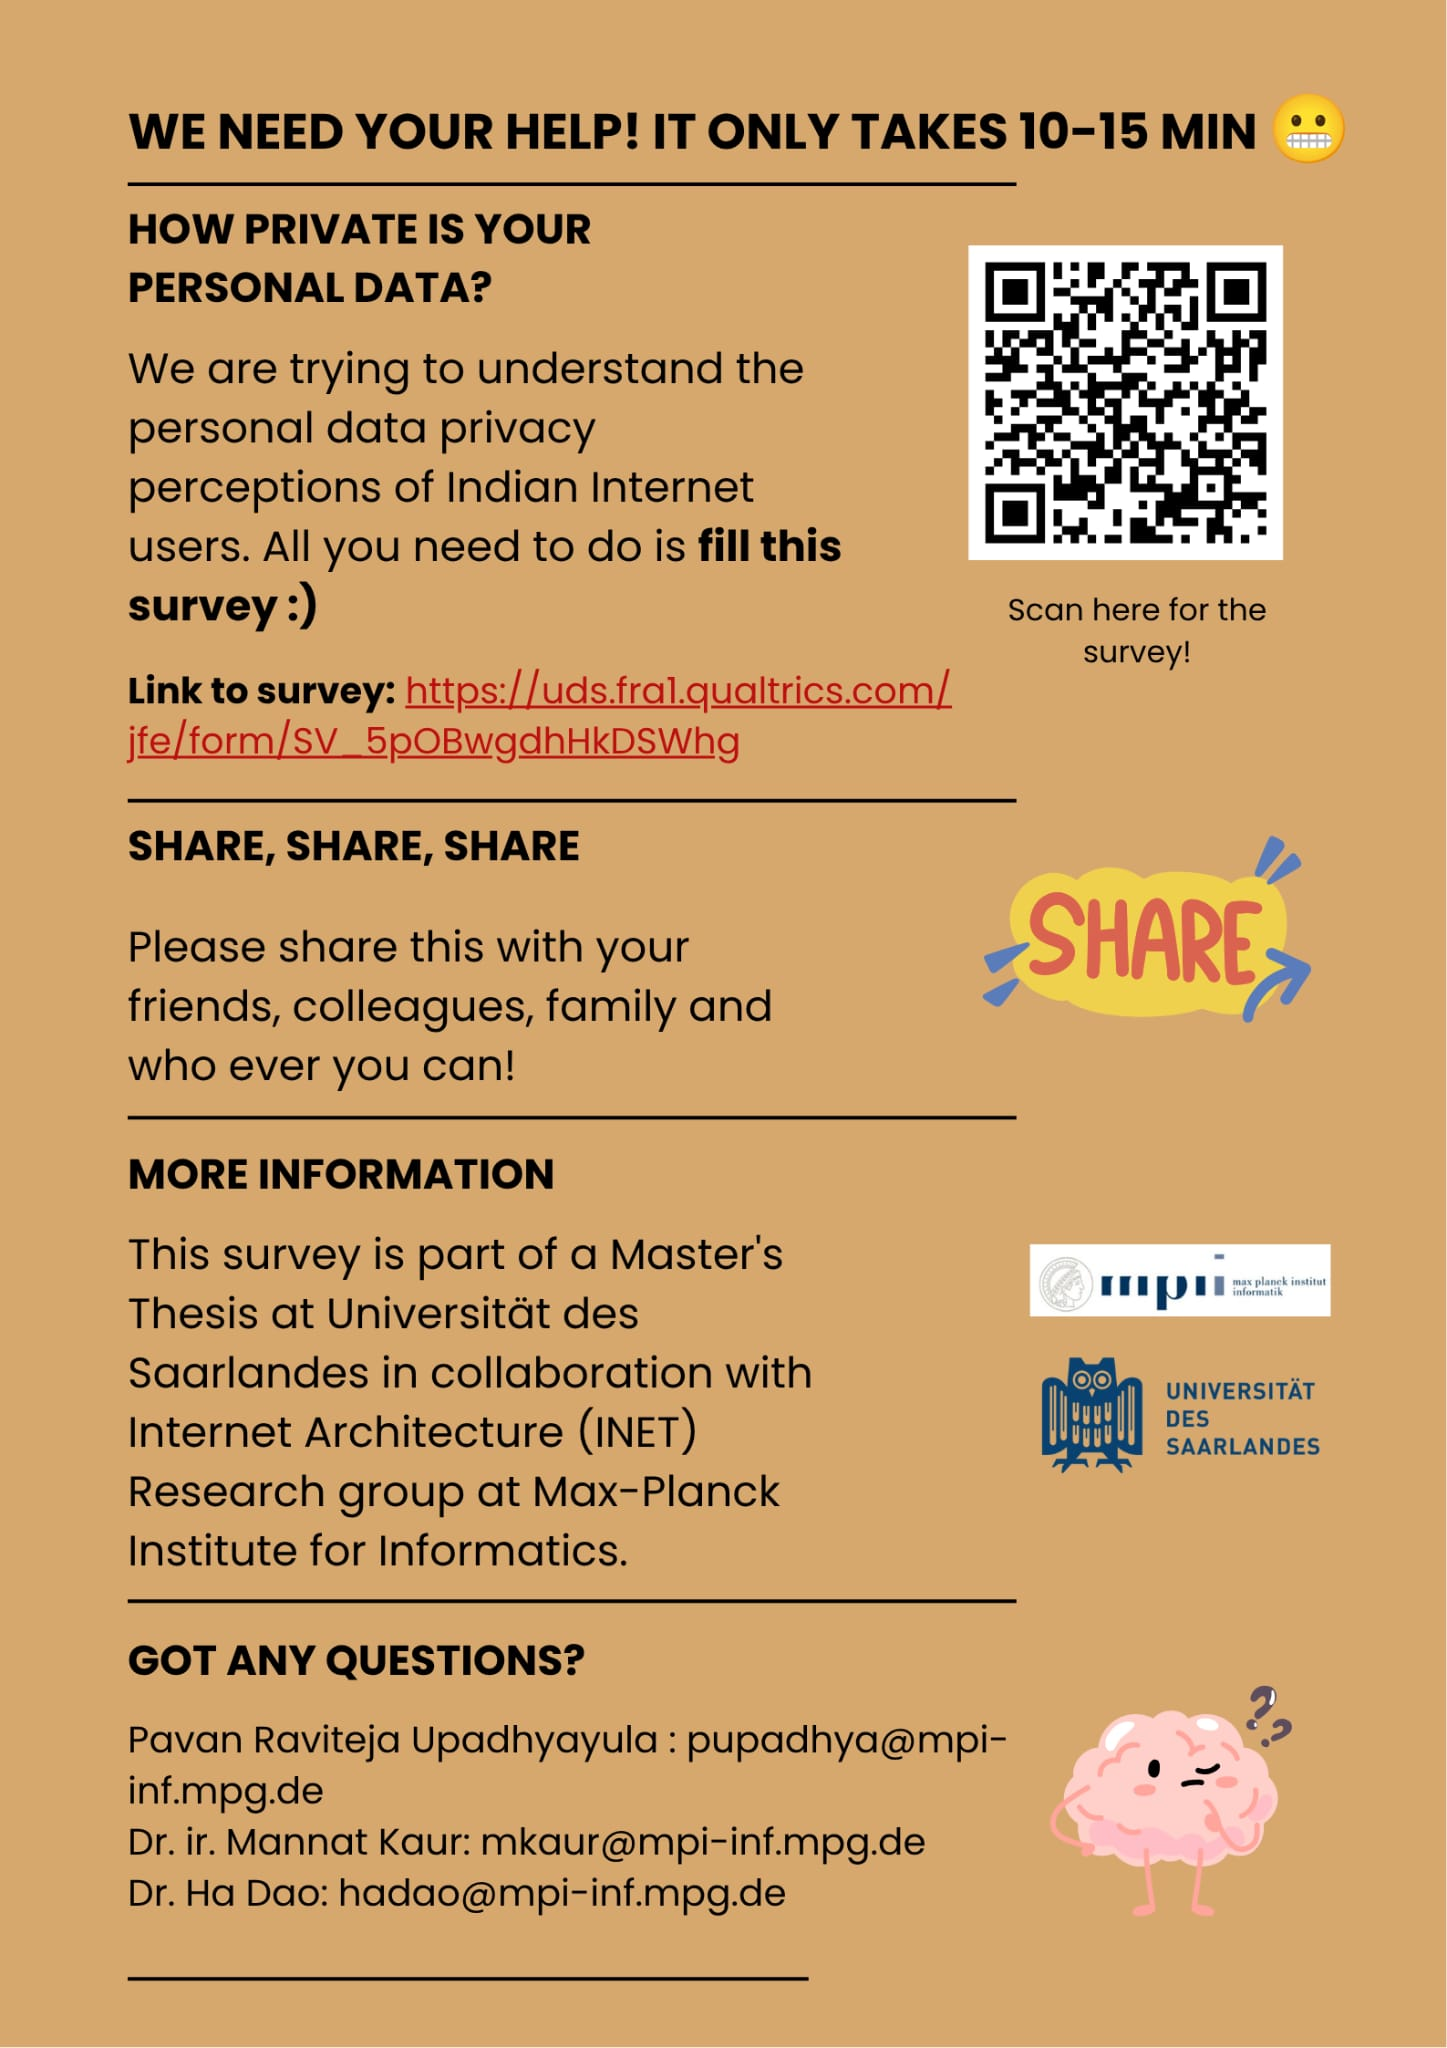
\includegraphics[width=0.7\linewidth]{Survey_poster.jpeg}
    \caption{Final study poster for recruitment}

\end{figure}

\renewcommand{\emph}{\textit}

\bibliographystyle{plainnat}
\bibliography{mybibliography}

\end{document}

%%% Local Variables:
%%% mode: latex
%%% TeX-master: t
%%% End:
